%% Files that are needed for LaTeX processing (style + inputs) are available
%% relative to the download place in the directory ../inputs, the images in
%% ../img

\documentclass[compress]{beamer}

\usepackage[utf8]{inputenc}
\mode<presentation>{
   \usetheme{BanjaLuka}
%   \usetheme{Warsaw}
   \hypersetup{pdfpagemode=FullScreen}
}
\setbeamertemplate{navigation symbols}{}

\usepackage{debian-links}

\title{Debian Teams Activity Metrics}

\author{Andreas Tille \& Sukhbir Singh}

%\institute{\Debian}
\institute{\link{http://www.debconf.org/debconf11/}{DebConf 11}}

\date{Banja Luka, July 29, 2011}

\begin{document}

\begin{frame}
  \titlepage
\end{frame}

\section{Short historical introduction}

\begin{frame}
  \frametitle{Motivation}
  \begin{itemize}
     \item Who is inside the team?
     \item Who left the team?
     \item Does a team have enough members?
     \item Is the team growing or shrinking?
  \end{itemize}
\end{frame}

\begin{frame}
  \frametitle{Quite simple start: Mailing list activity}
      \begin{center}
        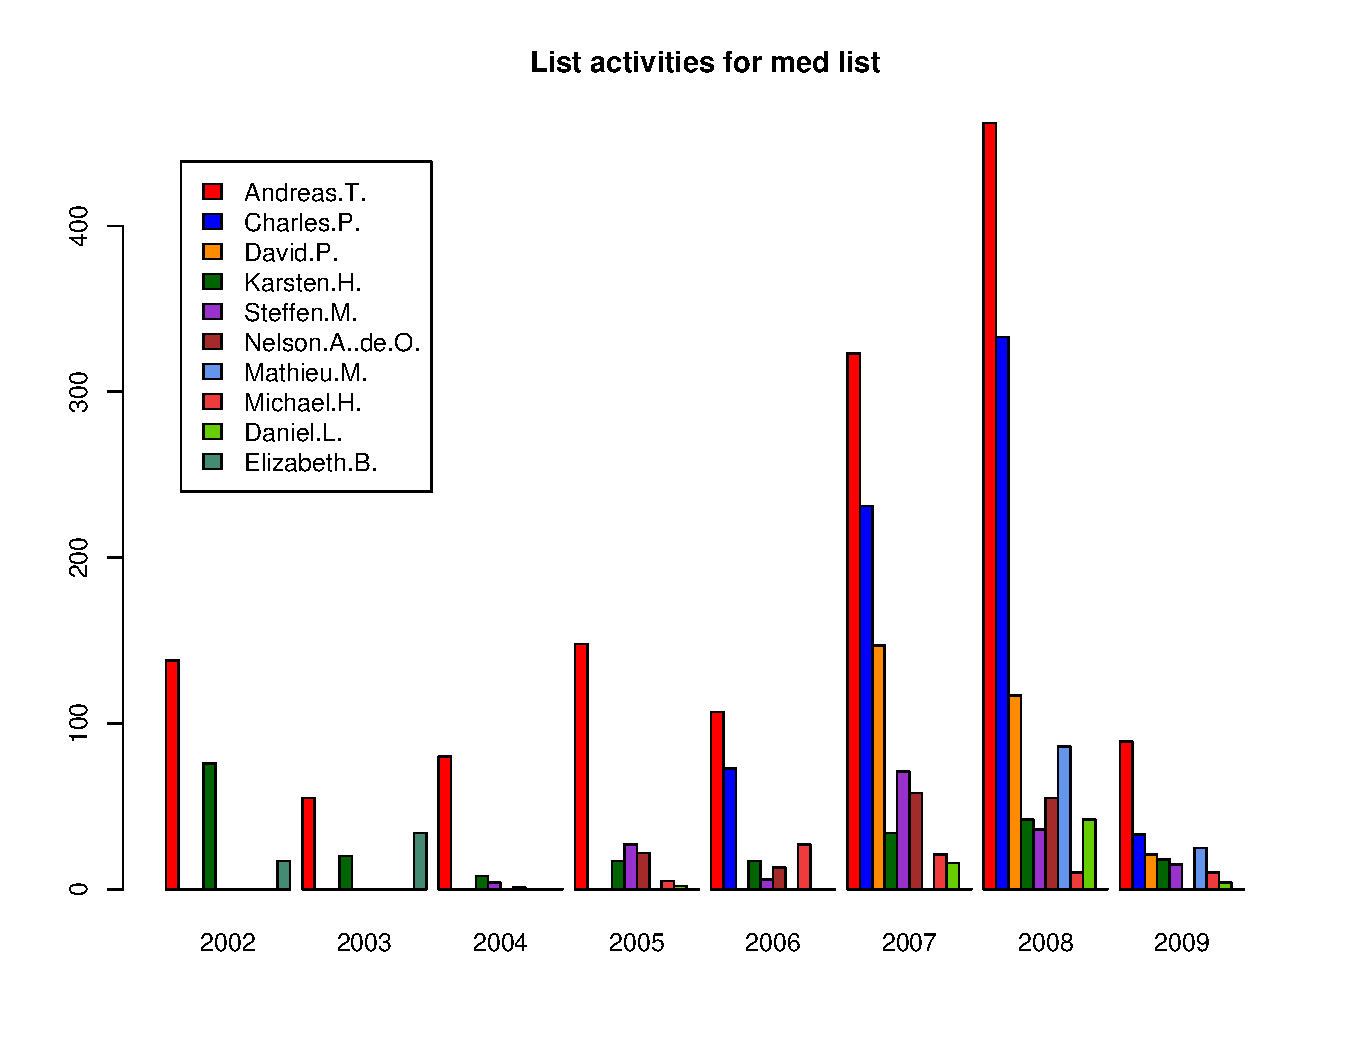
\includegraphics[width=0.9\textwidth]{authorstat_med}
      \end{center}
\end{frame}

\begin{frame}
  \frametitle{Enhancing the observation needed}
  \begin{itemize}
    \item We do not only want to know who is ``chatting''
    \item There should be a ``fair'' evaluation
    \item More flexibility
    \item Technical enhancements
  \end{itemize}
\end{frame}

\section{GSoC Project}

\begin{frame}
  \frametitle{Additional channels / means % FIXME
              to consider
             }
  \begin{itemize}
    \item VCS commits
    \item Uploaded packages
    \item Other ideas (IRC, \dots?)
  \end{itemize}
\end{frame}

\begin{frame}
    \frametitle{Implementation}
    \begin{itemize}
        \item We reinvented the wheel and wrote everything from scratch 
        \item \dots{} which makes it very easy for us to add new metrics or change existing ones
        \item The process is optimized because we perform remote operations for fetching repositories by SSHing into Alioth and performing them locally
        \item The code is pure Python (Python 2.6) and it's good and clean ;)
    \end{itemize}
\end{frame}

\begin{frame}
  \frametitle{Measure of Communication Activity}
  \begin{itemize}
     \item Every project has a mailing list
     \item We measure who are the most active contributors
     \item Quantity is not the only metric because quality matters 
     \item We handle spam by filtering it
  \end{itemize}
\end{frame}

\begin{frame}
  \frametitle{Quite simple start: Mailing list activity}
      \begin{center}
        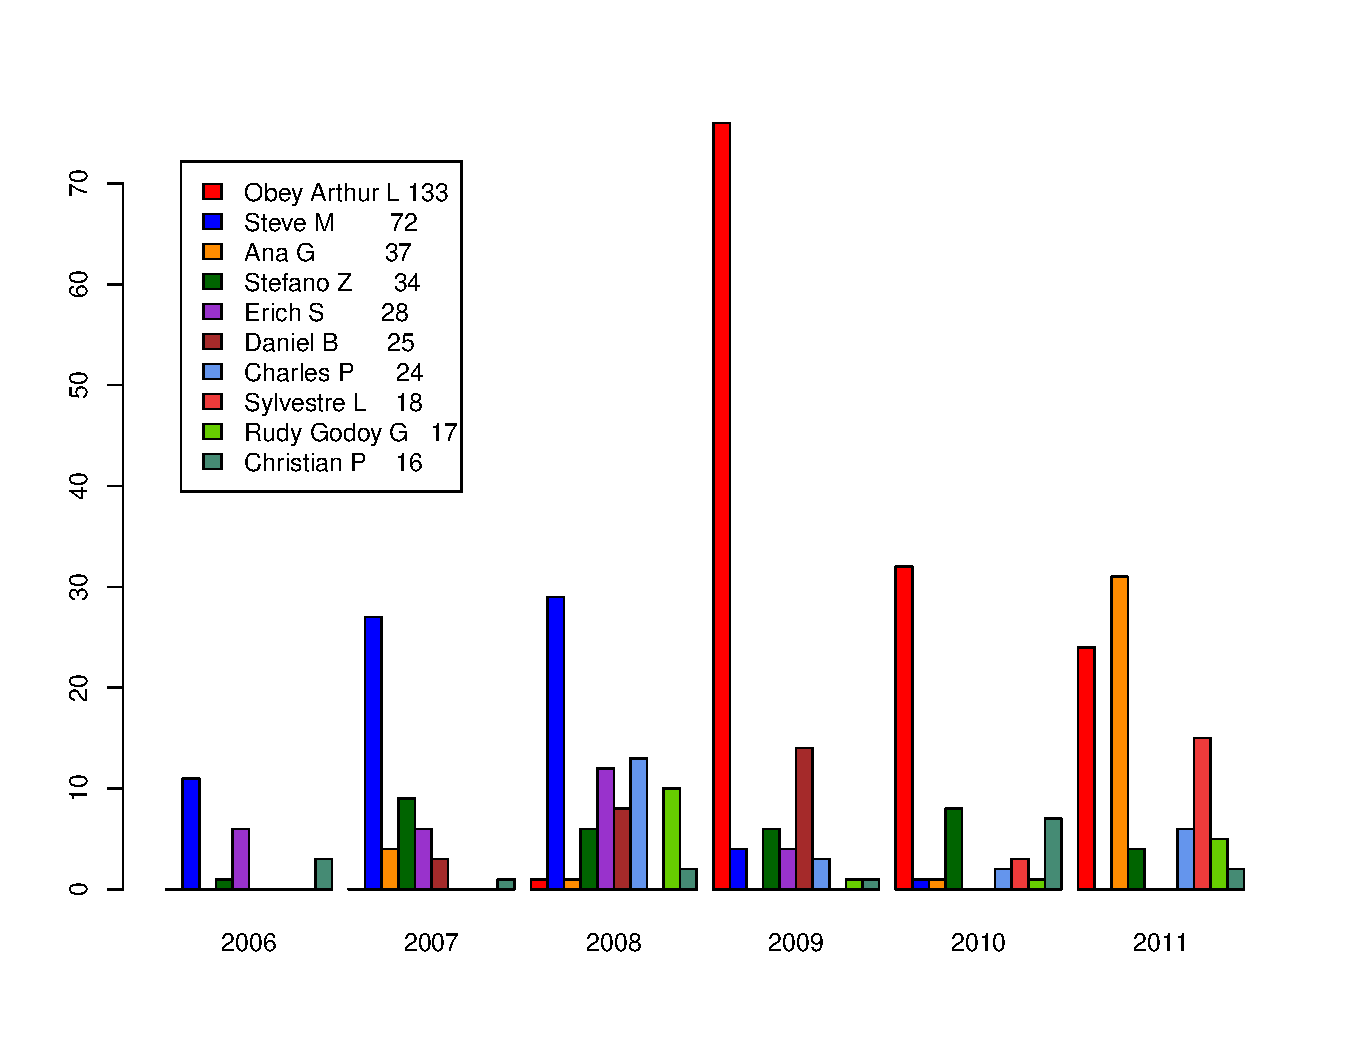
\includegraphics[width=0.9\textwidth]{authorstat_soc-coordination}
      \end{center}
\end{frame}

\begin{frame}
 \frametitle{Metrics for Measuring Communication Activity}
 \begin{itemize}
    \item Frequency of posting 
    \pause
    \item Message body metrics 
    \begin{itemize}
        \item the raw length of the message body
        \pause
        \item the length of the body \textit{excluding}
        \begin{itemize}
            \item blank lines
            \pause
            \item blank lines and quotes
            \pause
            \item blank lines, quotes and signatures
            \pause
        \end{itemize}
    \end{itemize}
    \pause
    \item Anything more that we can add? 
 \end{itemize}
\end{frame}

\begin{frame}
    \frametitle{Metrics for VCS}
    \begin{itemize}
        \item Frequency of commits for Git and SVN repositories
        \pause
        \item But again, quantity != quality
        \pause
        \item So we also measure the number of lines:
        \begin{itemize}
            \item (+) added
            \item (-) deleted
        \end{itemize}
    \end{itemize}
\end{frame}

\begin{frame}
    \frametitle{Noooooo!}
        \begin{center}
            
\includegraphics[scale=.25]{vaderno.jpg}
        \end{center}
        \begin{itemize}
            \item ``I find your using `lines of code commmitted' as a metric disturbing.''
            \pause
            \item Yes, Lord Vader, but then we don't have \textit{many} other metrics, so...
        \end{itemize}
\end{frame}

\begin{frame}
    \frametitle{Mailing list analysis: \textit{soc-coordination}}
\end{frame}

\begin{frame}
    \frametitle{Challenges}
    \begin{itemize}
    \item We don't have the mbox archives for lists.debian.org
        \begin{itemize}
        \pause
        \item So we fetch the archives through Gmane via NNTP, create mbox archives and then parse them
        \end{itemize}
    \pause
    \item How do we separate upstream commits for Git repositories on Alioth?
    \pause
    \item We need more metrics for measuring performance
    \pause
    \end{itemize}
    \center Please share your thoughts! 
\end{frame}

\begin{frame}
    \frametitle{Status}
    \begin{itemize}
        \item Complete
        \begin{itemize}
            \item Mailing list (Alioth, lists.debian.org)
            \item Repository (Git, SVN)
        \end{itemize}
    \end{itemize}

    \begin{itemize}
        \item Incomplete
        \begin{itemize}
            \item Package upload data from UDD
            \item Presenting these statistics
        \end{itemize}
    \end{itemize}
\end{frame}

\begin{frame}
    \frametitle{Questions? Suggestions?}
    \begin{center}
    The more we discuss, the better we can get!
    \end{center}
    \begin{center}
    Join us: http://teammetrics.alioth.debian.org/
    \end{center}
\end{frame}

\end{document}
